\subsection{Applikation}

\subsubsection{Funktion}

Die Applikation ist ein eigenständiges Programm.
Dieses kommuniziert mit dem Treiber über \gls{ioctl}.
Das Programm ist in \textit{Python 3} implementiert.
Das Programm ließt periodisch einen Temperatur-Messwert $\texttt{M}_C[n]$ in \si{\celsius} aus und bildet diesen zu einem \gls{pwm}-Duty-Cycle $\texttt{D}[n]$ nach dem Prinzip von \autoref{eq:app} um.
Da der Treiber die Abtastrate weder vorgibt, noch künstlich limitiert, kann die Samplingfrequenz durch die Applikation frei gewählt werden.
Der Parameter $n$ steht hier für die Nummer eines Samples.
\begin{equation}
    g \left( \texttt{M}_C \left[n\right] \right) \rightarrow \texttt{D}\left[n\right]
    \label{eq:app}
\end{equation}

Grundsätzlich kann die Übertragungsfunktion $g$ beliebig implementiert werden.
Diese kann sogar von historischen Messdaten $\texttt{M}_C[n-m]$ abhängig sein.
Dabei ist der Parameter $m$ ein beliebiger Offset in die Vergangenheit.
Damit bleibt sowohl die Einfachheit der Nutzung, als auch die Flexibilität komplexe Signalverarbeitung zu betreiben, bestehen.
Unsere Implementation realisiert zur Demonstration einen einfachen, kontextfreien, \gls{lut}.
Dieser beinhaltet einzelne Eingabe/Ausgabe Wert-Datenpaare aus einer \gls{csv} Datei und bestimmt den momentanen Ausgang anhand von linearer Interpolation am Eingangswert.
Die resultierende Übertragungsfunktion ist eine stückweise lineare Funktion.
Ein Beispiel dafür ist in \autoref{fig:pcl} mit den Datenpunkten aus Tabelle \ref{tab:pcl} dargestellt.
% No Autoref, since autoref uses the name of the parent element and thus calls the table a figure

\begin{figure}[h]
    \centering
    \begin{subfigure}[b][][t]{9cm}
        \centering
        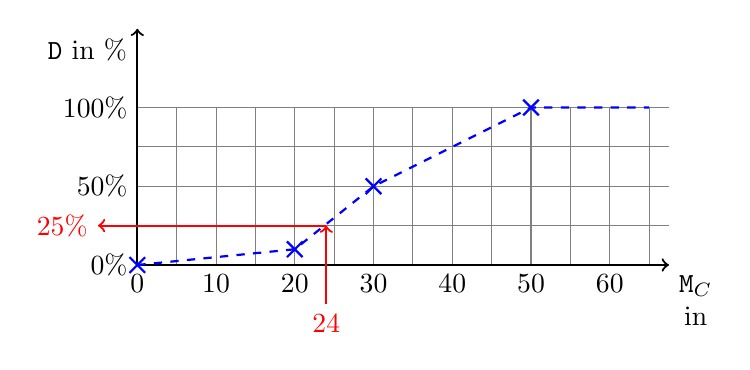
\begin{tikzpicture}
            \draw[step=0.5,gray,thin] (0,0) grid (6.75,2);
            \draw[thick, ->] (0,0) -- ++(6.75,0) node[below right, align=center] {$\texttt{M}_C$\\ in \si{\celsius}};
            \draw[thick, ->] (0,0) -- (0,3) node[below left] {$\texttt{D}$ in \%};
            \draw (0,0) node[left]  {$0\%$};
            \draw (0,1) node[left]  {$50\%$};
            \draw (0,2) node[left]  {$100\%$};
            \draw (0,0) node[below] {$0\si{\degree}$};
            \draw (1,0) node[below] {$10\si{\degree}$};
            \draw (2,0) node[below] {$20\si{\degree}$};
            \draw (3,0) node[below] {$30\si{\degree}$};
            \draw (4,0) node[below] {$40\si{\degree}$};
            \draw (5,0) node[below] {$50\si{\degree}$};
            \draw (6,0) node[below] {$60\si{\degree}$};
            \draw[thick, blue] plot[mark=x, mark size=4pt, only marks] coordinates {(0,0) (2,0.2) (3, 1) (5,2)};
            \draw[thick, blue, dashed] plot[] coordinates {(0,0) (2,0.2) (3, 1) (5,2) (6.5,2)};
            \draw[thick, red, ->] (2.4, 0.5) -- (-0.5,0.5) node[left] {\textcolor{red}{$25\%$}};
            \draw[thick, red, ->] (2.4, -0.5) node[below] {\textcolor{red}{$24\si{\celsius}$}} -- (2.4,0.5);
        \end{tikzpicture}
        \caption{Applikations \acrshort{lut} Beispiel. Die \textcolor{blue}{blauen Punkte} bilden den \gls{lut}. Die \textcolor{blue}{blaue Linie} zeigt die lineare interpolation. Die \textcolor{red}{rote Intersektion} zeigt einen Beispielswert und dessen dazugehöriges Interpolationsresultat an.}
        \label{fig:pcl}
    \end{subfigure}
    \quad
    \begin{subtable}[b][][t]{3.5cm}
        \centering
        \begin{tabular}{|l|l|}
            \hline
            \textbf{$\texttt{M}_C$ in $\si{\celsius}$} & \textbf{$\texttt{D}$ in $\%$} \\
            \hline
            \hline
            0 & 0 \\
            \hline
            20 & 20 \\
            \hline
            30 & 50 \\
            \hline
            50 & 100 \\
            \hline
        \end{tabular}
        \vspace{0.75cm}
        \caption{Beispieldaten für die Übertragungsfunktion aus \autoref{fig:pcl}.}
        \label{tab:pcl}
    \end{subtable}
    \caption{Applikations \acrshort{lut} Beispiel}
\end{figure}

\subsubsection{\acrshort{ipc} über \acrshort{ioctl}}

\textit{Python} unterstützt \gls{ioctl} durch die \texttt{fcntl} Standardbibliothek.
Jedoch existieren die C-Makros zur Definition der \gls{ioctl} Konstanten nicht.
Dazu wird die externe \textit{ioctl\_opt}\cite{ioctl} Bibliothek benutzt.
Diese in Kombination der Standard \textit{ctypes} Bibliothek ermöglicht eine ähnliche Nutzung zu den Nativen C-Makros.
Die \textit{ioctl\_opt} Bibliothek stellt ähnliche Makros zur Verfügung.
Die interne Implementation besteht aus logischen Operationen und Shifts.
Die resultierenden \gls{ioctl} Konstanten können danach auf eine geöffnete Instanz der Pseudodatei in \texttt{/etc/fanctrl} durch \texttt{fcntl.ioctl} mit einem geeigneten Buffer angewendet werden.
Um den Buffer zu schreiben oder zu lesen wird die native \texttt{Bytes} Klasse verwendet.
Die Bytes benutzen \textit{little Endianness}.
Eine relevante Funktion ist in \autoref{code:py-ioctl} aufgeführt.

\lstinputlisting[linerange={27-36}, firstnumber=27, caption={\texttt{./app/app.py} \gls{ioctl} zum Auslesen der Temperatur}, language=python, label=code:py-ioctl, float=h]{../../app/app.py}

\subsubsection{Installation und Ausführung}

Zur Ausführung wird eine globale Instanz von \textit{Python} Version \texttt{3.x.x} benötigt.
Es werden externe Abhängigkeiten benötigt.
Es wird empfohlen diese in ein lokales \texttt{virtual environment} zu installieren um den globalen Scope nicht zu vermüllen.
Der empfohlene Prozess zur Ausführung ist in \autoref{code:install} angegeben.

\begin{lstlisting}[
    language=bash, numbers=none,
    label=code:install,
    caption={Installationsvorgang der Applikation}
]
cd app
python3 -m venv venv
source ./venv/bin/activate
pip install -r requirements.txt
chmod +x ./app.py
./app.py
\end{lstlisting}
